% !TeX TXS-program:compile = txs:///pdflatex/[--shell-escape]



% #######################################
% ######### Параметры документа #########
% #######################################

% 14-й шрифт (стандарт для дипломных работ) %
\documentclass[a4paper,14pt]{extarticle}
% 12-й шрифт %
%\documentclass[12pt, a4paper]{article}

% Кодировки требуются только если компилятор не включает поддержку Unicode
% (поддержку по умолчанию имеют XeTeX, LuaLaTeX)
\usepackage[utf8x]{inputenc}
\usepackage[T1, T2A]{fontenc}
\usepackage[english,russian]{babel}

% Стилевой файл %
\usepackage[spisok,boldsect,eqwhole,figwhole,hyperref,hyperprint,greekit]{fn2style/fn2kursstyle}

% Междустрочный интервал 1.5 %
\usepackage{setspace}
\setstretch{1.5}

% Размер полей %
\usepackage[left=3cm,right=1cm, top=2cm,bottom=2cm]{geometry}

% Включение титульника PDF %
\usepackage{pdfpages}

% Меняем нумерацию страниц с красивой на снизу по центру %
\pagestyle{plain}

% multline внутри других оболочек %
\usepackage{mathtools}

% Центрированные таблицы фиксированной ширины %
\usepackage{tabularx} % also loads 'array' package
\newcolumntype{C}{>{\centering\arraybackslash}X} % centered version of 'X' columns

% 2-я страница оглавления начинается без отступа сверху %
\usepackage[titles]{tocloft}
% Т.е. используем tocloft, требуется явно указать что основные разделы заполняют простанство до станиц точками %
\renewcommand{\cftsecleader}{\cftdotfill{\cftdotsep}}

% Фикс для false-positive warning'ов из bibliography %
% (bibliography использует \sloppy чтобы несколько ослабить правила переноса, но \sloppy не трогает анализатор hbadness, который начинает давать false-positive предупреждения о "некрасивых" переносах строки) %
\usepackage{etoolbox}
\apptocmd{\sloppy}{\hbadness 10000\relax}{}{}

% Делаем verbatim меньше %
\usepackage{verbatim}

\newenvironment{smallverbatim}%
{\small\verbatim}%
{\endverbatim}

\newenvironment{tinyverbatim}%
{\footnotesize\verbatim}%
{\endverbatim}

% Путь к графике %
\graphicspath{{./style/}{./images/}}



% ######################################
% ######### Кастомные комманды #########
% ######################################

% d %
\newcommand*\diff{\mathop{}\!\mathrm{d}}
% 1/2 %
\newcommand{\half}{{1/2}}
% Div %
\renewcommand{\div}{\mathrm{div}}
% Grad %
\newcommand{\grad}{\mathrm{grad}}
% Const %
\newcommand{\const}{\mathrm{const}}
% E %
\newcommand{\E}{\mathbb{E}}
% D %
\newcommand{\D}{\mathbb{D}}
% D %
\newcommand{\K}{\mathbb{K}}
% = by def %
\newcommand\eqbydef{\mathrel{\overset{\makebox[0pt]{\mbox{\normalfont\tiny\sffamily def}}}{=}}}
% epsilon %
\renewcommand{\epsilon}{\varepsilon}
% Re %
\renewcommand{\Re}{\ensuremath{\,\textrm{Re}}}
% Im %
\renewcommand{\Re}{\ensuremath{\,\textrm{Im}}}
% Vector %
\renewcommand{\vec}{\bi}
% e %
\newcommand{\euler}{\mathrm{e}}
% dirac delta %
\newcommand{\diracdelta}{\delta}
% green function G %
\newcommand{\greenfunc}{\mathrm{G}}
% erf %
\newcommand{\erf}{\mathrm{erf}}
% Wide tilde %
\newcommand{\wt}{\widetilde}
% Wide tilde %
\newcommand{\forany}{\forall}

% Запятая в индексах
\newcommand{\idxcomma}{,\;}

% Shortcut для дифференцирования по 1 аргументу

\newcommand{\dpartial}[2]{\dfrac{\partial #1}{\partial #2}}

\newcommand{\dfull}[2]{\dfrac{\diff #1}{\diff #2}}

% Маленький верхний индекс %
\usepackage{relsize}
\newcommand{\smallalpha}{\mathsmaller{(} \alpha \mathsmaller{)}}
\newcommand{\smallbeta}{\mathsmaller{(} \beta \mathsmaller{)}}

% Осреднение по ансамблю %
\newcommand{\avg}[1]{\left\langle #1 \right\rangle}

% Временные комментарии %
\newcommand{\intextnote}[2]{\begin{center}{\color{#2}\textbf{
	\rule{\textwidth}{2.0pt}
	\\ #1 \\
	\rule{\textwidth}{2.0pt}
}}\end{center}}

\newcommand{\COMMENT}[1]{\intextnote{#1}{red}}
\newcommand{\NOTE}[1]{\intextnote{#1}{blue}}

\newcommand{\appwidth}{6.45cm}

% {gather} для использования в тексте - не добавляет вертикальных пробелов %
\newenvironment{inlinegather*}{\par\centering$\displaystyle\begin{aligned}}{\end{aligned}$\par}


% ~~~~~~~~~~~~~~~~~~~~~~~~~~~~~~~~~~~~~~~~~~~~~~~~~~~~~~~~~~~~~~~~~~~~~~~~~~~~~~~~~~~~~~~~~~~~~~~~~~~~~~

\begin{document}

\title{"Методы численного решения задача линейной алгебры"}
\group{ФН2\,--\,31М}
\author{Д.\,И.~Богданов}
\supervisor{А.\,С.~Родин}
\date{2024}
\maketitle

% ==================
% --- Оглавление ---
% ==================

\newpage
\tableofcontents
\newpage


\section{Постановка задачи}


Нужно сформировать матрицу размером $10 \times 10$ по следующему принципу. В качестве базовой матрицы $А$, берется известная матрица, которая получается после дискретизации одномерного оператора Лапласа методом конечных разностей или методом конечных элементов. На равномерной сетке:
\[
A_0 = \left\lbrace a_{ij} \right\rbrace_{i, j = \overline{1, n}}
\]
где
\[
a_{ij} = \begin{cases}
2, \quad &i = j, \\
-1, \quad &|i-j| = 1, \\
0, \quad &\text{else}. \\
\end{cases}
\]
Для данной матрицы известны аналитические формулы для собственных значений ($n = 10$)
\[
\lambda_j^0 =2 (1 - \cos \dfrac{\pi j}{n + 1}),
\quad j = \overline{1, n}.
\]
и компонент собственных векторов (вектора имеют $2$-норму равную $1$):
\[
z_j^0 (k) = \sqrt{\dfrac{2}{n+1}} \sin \dfrac{\pi j k}{n+1},
\quad k = \overline{1, n}.
\]
Итоговая матрица получается по формулам:
\begin{gather*}
A = A_0 + \delta A, \\
\delta A_{ij} = \begin{cases}
\dfrac{c}{i + 1}, \quad &i \neq j, \\
0, \quad &i = j,
\end{cases} \\
c = \dfrac{N_{var}}{N_{var} + 1} \epsilon.
\end{gather*}
где $N_{var}$ --- номер варианта (совпадает с номером студента в списке в журнале
группы), $\epsilon$ - параметр, значение которого задается далее.

Нужно выполнить следующие задания:

\subsection{Задание 1}

Взять матрицу $А$ для значения $\epsilon = 0.1$, убрать последний столбец и сформировать из первых $9$ столбцов матрицу $\hat{A}$ размера $10 \times 9$. Решить линейную задачу наименьших квадратов для вектора невязки
\[
r = \hat{A} x - b,
\]
где вектор $b$ размерности $10 \times 1$ нужно получить по следующему алгоритму: выбрать вектор $x_0$, размерности $9 \times 1$ и для него вычислить $b = \hat{А} х_0$.

Для решения поставленной задачи использовать QR разложение: для вариантов с четным номером использовать соответствующий алгоритм, основанный на методе вращений Гивенса, для вариантов с нечетным номером - алгоритм, основанный на методе отражений Хаусхолдера.

После получения решения сделать оценку величины $|| x - x_0 ||_2 / ||x_0||_2$.

\subsection{Задание 2}

Для матрицы $А$ найти все ее собственные значения ($\lambda_j, j = \overline{1, 10}$) и собственные вектора ($z_j, j = \overline{1, 10}$, с $2$-нормой равной $1$) с помощью неявного QR-алгоритма со сдвигом (с предварительным приведением матрицы к форме Хессенберга) для трех вариантов: $\epsilon = 10^{-1}, 10^{-3}, 10^{-6}$.

По итогам расчетов нужно сделать сводную таблицу, в которой указать следующие величины: $\lambda_j - \lambda_j^0$ и $||z_j - z_j^0||_2$ для $j = \overline{1, 10}$.

\section{Решение линейной задачи наименьших квадратов в с помощью QR-разложения методом отражений Хаусхолдера}

В рамках данной задачи реализованы следующие алгоритмы:
\begin{itemize}
\item Отражение Хаусхолдера;

\item Обычное QR-разложение;

\item QR-разложение для метода LLS;

\item Обратный ход метода Гаусса;

\item Linear Least Squares с помощью QR-разложения.
\end{itemize}

Расчетная реализация всех алгоритмов выполнена на языке \texttt{C++} с использованием библиотеки \texttt{Eigen} для базовых матричных операций. Для отладки программы и проверки корректности результатов реализован вспомогательный скрипт на \texttt{Wolfram Mathematica}, использующий встроенные методы для получения необходимых разложений.

Изначальная форма алгоритма QR-разложения имеет следующий вид:
\begin{smallverbatim}
----------------------------------------------------------------------
-   Q_wave = I;                                                      -
-   R_wave = A;                                                      -
-   for i = 1,min(M-1,N) {                                           -
-      ui                = House(R_wave[i:M, i])      // O(N)        -
-      pi_wave           = I - 2 ui ui^T              // O(N^2)      -
-      pi                = I                          //             -
-      pi[i:M, i:M]      = pi_wave                    //             -
-      R_wave[i:M, i:N]  = pi_wave * R_wave[i:M, i:N] // O(N^3)      -
-      Q_wave[0:M, i:M]  = Q_wave[0:M, i:M] * pi_wave // O(N^3)      -
-   }                                                                -
-   return { Q[0:M, 0:N], R[0:N, 0:N] }                              - 
----------------------------------------------------------------------
\end{smallverbatim}

В явном виде алгоритм имеет сложность $O(N^4)$, это решается если подставить матрицу $p_i$ явно и расписать матричное умножение как $2$ умножения матрицы на вектор. Приходим к следующему алгоритму:

\begin{smallverbatim}
----------------------------------------------------------------------
-   Q_wave = I;                                                      -
-   R_wave = A;                                                      -
-   for i = 1,min(M-1,N) {                                           -
-      ui                = House(R_wave[i:M, i])          // O(N)    -
-      R_wave[i:M, i:N] -= 2 ui (ui^T * R_wave[i:M, i:N]) // O(N^2)  -
-      Q_wave[0:M, i:M]  -= Q_wave[0:M, i:M] * 2 ui ui^T  // O(N^2)  -
-   }                                                                -
-   return { Q[0:M, 0:N], R[0:N, 0:N] }                              -
----------------------------------------------------------------------
\end{smallverbatim}

Произведено тестовое QR-разложение матрицы $\hat{A}$, проверена ортогональность матрицы $Q$ и приблизительное совпадение $QR \approx A$. Результаты сходятся с разложением с помощью встроенного метода \texttt{QRDecomposition[ ]} в пакете \texttt{Wolfram Mathematica}.

Модификация QR-разложени для метода LLS также позволяет вычислять правую часть $Q^T b$ сразу по ходу разложения с целью экономии вычислительных ресурсов. Алгоритм описан в листинге программы

В качестве тестового вектора выбран $x_0: x_i = i^2$. Для него решена задача наименьших квадратов относительно невязки, получен вектор $x_{LLS}$ имеющий следующую норму ошибки:
\begin{verbatim}
lls_error_estimate -> 3.990082657206211e-16
\end{verbatim}

Результаты LLS также сверены с помощью скрипта.

\section{Получение собственных значений матрицы с помощью QR-алгоритма со сдвигами}

В рамках данной задачи реализованы следующие алгоритмы:
\begin{itemize}
\item Приведение матрицы к Хессенберговой форма;

\item QR-алгоритм без сдвигов (для отладочных целей);

\item $O(N^2)$ QR-разложение для верхне-хессенберговых матриц с вычислением $RQ$;

\item QR-алгоритм со сдвигами и приведением изначальной матрицы к Хессенберговой форме;
\end{itemize}

В качестве значений сдвига в QR-алгоритме берется $H_{nn}$, итерации производятся до тех пор пока значение $|H_{n, n-1}|$ не станет меньше некоторого $\epsilon$, после чего $n$-е значение на диагонали считаем найденым и редуцируем задачу к работе с блоком $(n - 1) \times (n - 1)$. Процедура повторяется до достижения максимального числа итераций или редукции $n$ к $2$-м (при нормальном ходе программы ожидается второй исход). Приходим к следующему алгоритму:

\begin{smallverbatim}
---------------------------------------------------------------------------
-   while (N >= 2 && iteration++ < max_iterations) {                      -
-      sigma = T_shur[N, N]                                     // O(1)   -
-      [ Q, R, RQ ] = qr_factorize_hessenberg(T_shur[1:N, 1:N]) // O(N^2) -
-      T_shur[0:N, 0:N] = RQ + sigma I                          // O(N^2) -
-      if (|T_shur[N, N-1]| < eps) --N                          // O(1)   -
-   }                                                                     -
---------------------------------------------------------------------------
\end{smallverbatim}

Таким образом, метод редуцируется к сложности $O(N^3)$, без учета хессенберговой структуры имели бы $O(N^4)$. Матрицы $Q$, $R$ в данной реализации не нужны в явном виде, однако программно также определяются для отладочных целей.

В результате работы алгоритма получаем матрицу $T$ из разложения Шура, значения на главной диагонали соответствуют собственным значениям изначальной матрицы.

Получены собственные значения матрицы $A$, результаты сравнения с аналитическими результатами приведены ниже для $\epsilon = 10^{-1}, 10^{-3}, 10^{-6}$:
\begin{center}
\begin{tabular}{|c|c|c|}
\hline
 j & $|\lambda_j^0 - \lambda_j|$ & $||z_j^0 - z_j||_2$ \\
\hline
 1 &  0.0383792 & x \\
 2 & 0.00164998 & x \\
 3 & 0.00198987 & x \\
 4 & 0.00445514 & x \\
 5 & 0.00474202 & x \\
 6 & 0.00674079 & x \\
 7 & 0.00682261 & x \\
 8 & 0.00718661 & x \\
 9 & 0.00664725 & x \\
10 & 0.00542461 & x \\
\hline
\end{tabular}
\captionof{table}{Ошибки при $\epsilon = 10^{-1}$}
\end{center}

\begin{center}
\begin{tabular}{|c|c|c|}
\hline
 j & $|\lambda_j^0 - \lambda_j|$ & $||z_j^0 - z_j||_2$ \\
\hline
 1 & 0.000395515 & x \\ 
 2 & 1.15997e-05 & x \\ 
 3 & 1.46055e-05 & x \\ 
 4 & 4.50412e-05 & x \\ 
 5 & 4.80620e-05 & x \\ 
 6 & 6.73953e-05 & x \\ 
 7 & 6.82741e-05 & x \\ 
 8 & 7.18550e-05 & x \\ 
 9 & 6.65622e-05 & x \\ 
10 & 5.45308e-05 & x \\ 
\hline
\end{tabular}
\captionof{table}{Ошибки при $\epsilon = 10^{-1}$}
\end{center}

\begin{center}
\begin{tabular}{|c|c|c|}
\hline
 j & $|\lambda_j^0 - \lambda_j|$ & $||z_j^0 - z_j||_2$ \\
\hline
 1 & 3.95623e-07 & x \\
 2 & 1.15569e-08 & x \\
 3 & 1.45556e-08 & x \\
 4 & 4.50458e-08 & x \\
 5 & 4.80682e-08 & x \\
 6 & 6.73952e-08 & x \\
 7 & 6.82745e-08 & x \\
 8 & 7.18549e-08 & x \\
 9 & 6.65631e-08 & x \\
10 & 5.45337e-08 & x \\
\hline
\end{tabular}
\captionof{table}{Ошибки при $\epsilon = 10^{-1}$}
\end{center}

Пример сводки результатов расчета для малого $n$ (в силу вербозности результата при $n = 10$) приведен в приложении.

% includepdf омерзительно кривой, поэтому заголовки приходится ставить так

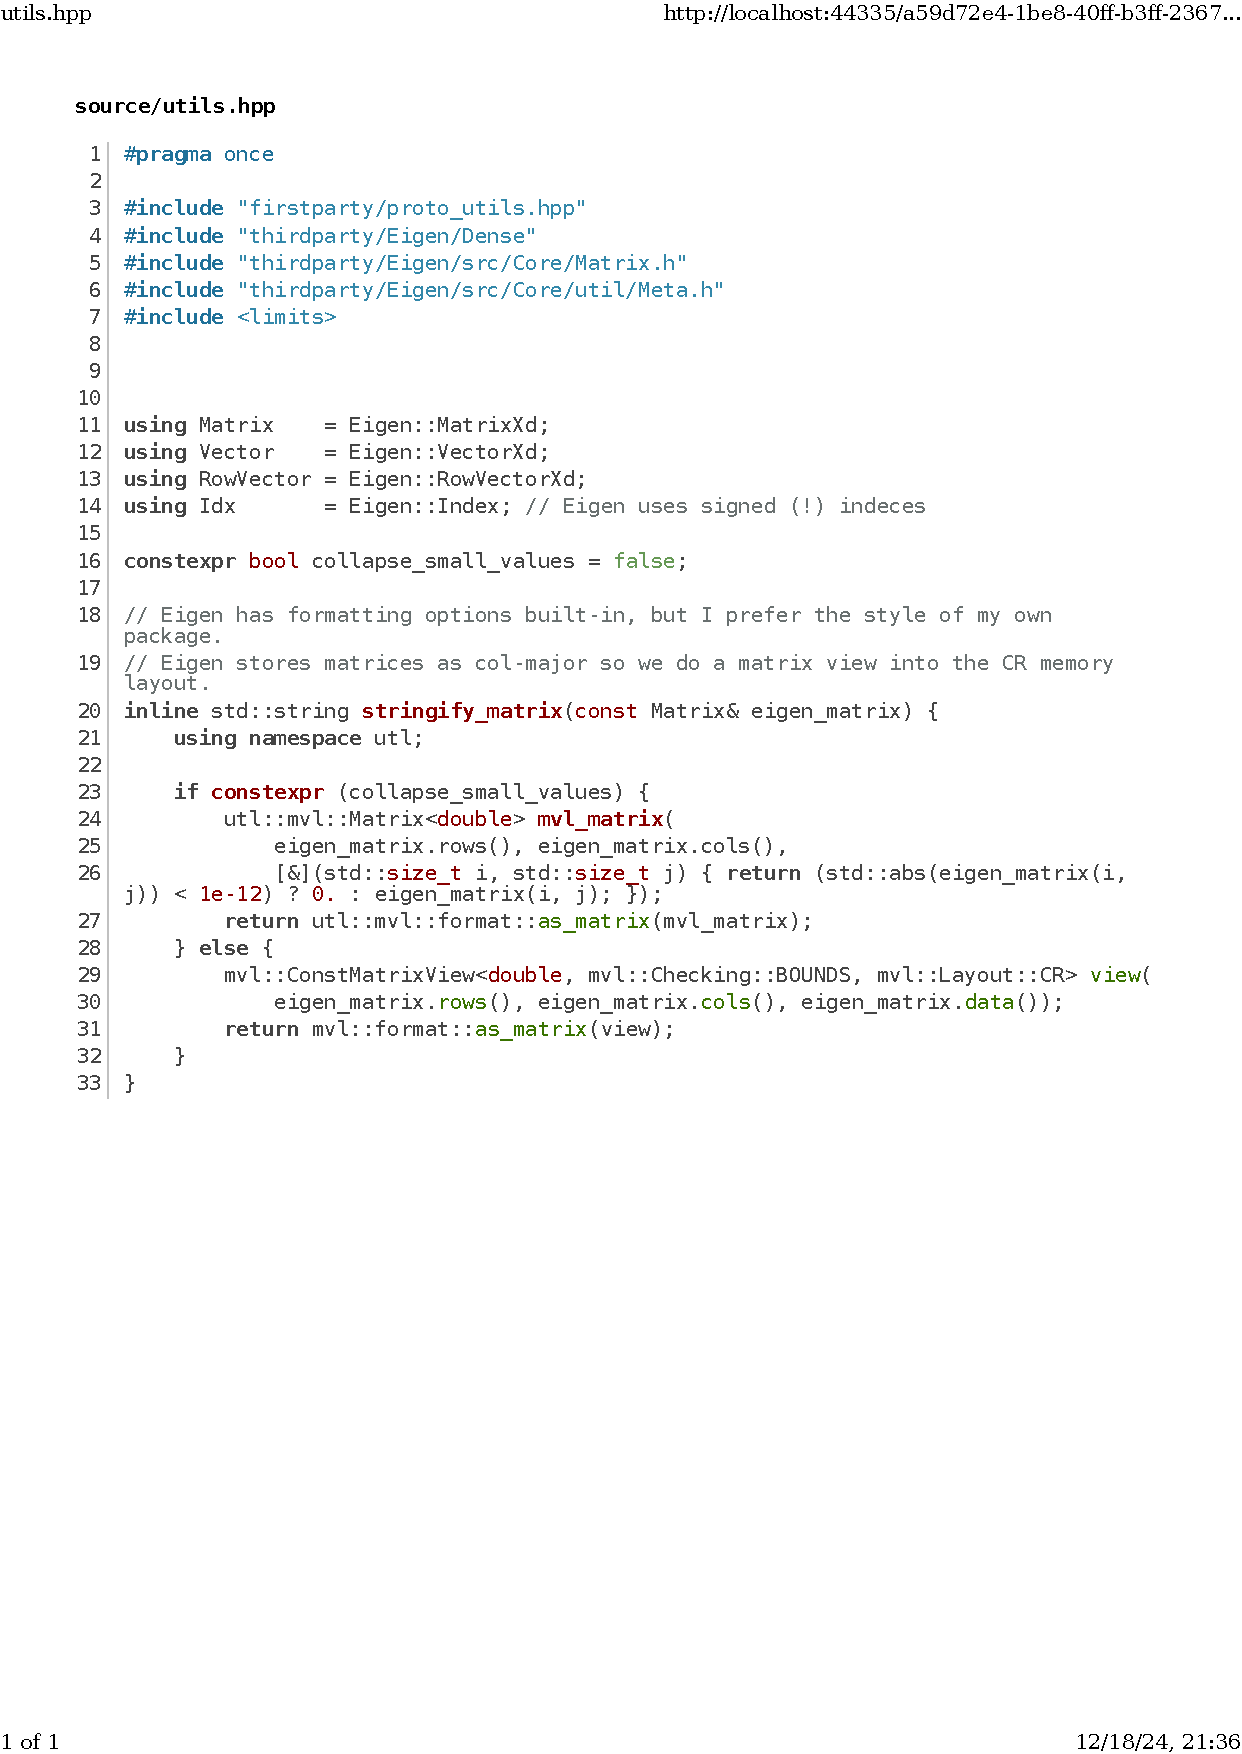
\includepdf[scale=0.9,pagecommand=\section{Листинг расчетной программы на C++}]{images/utils.hpp.pdf}
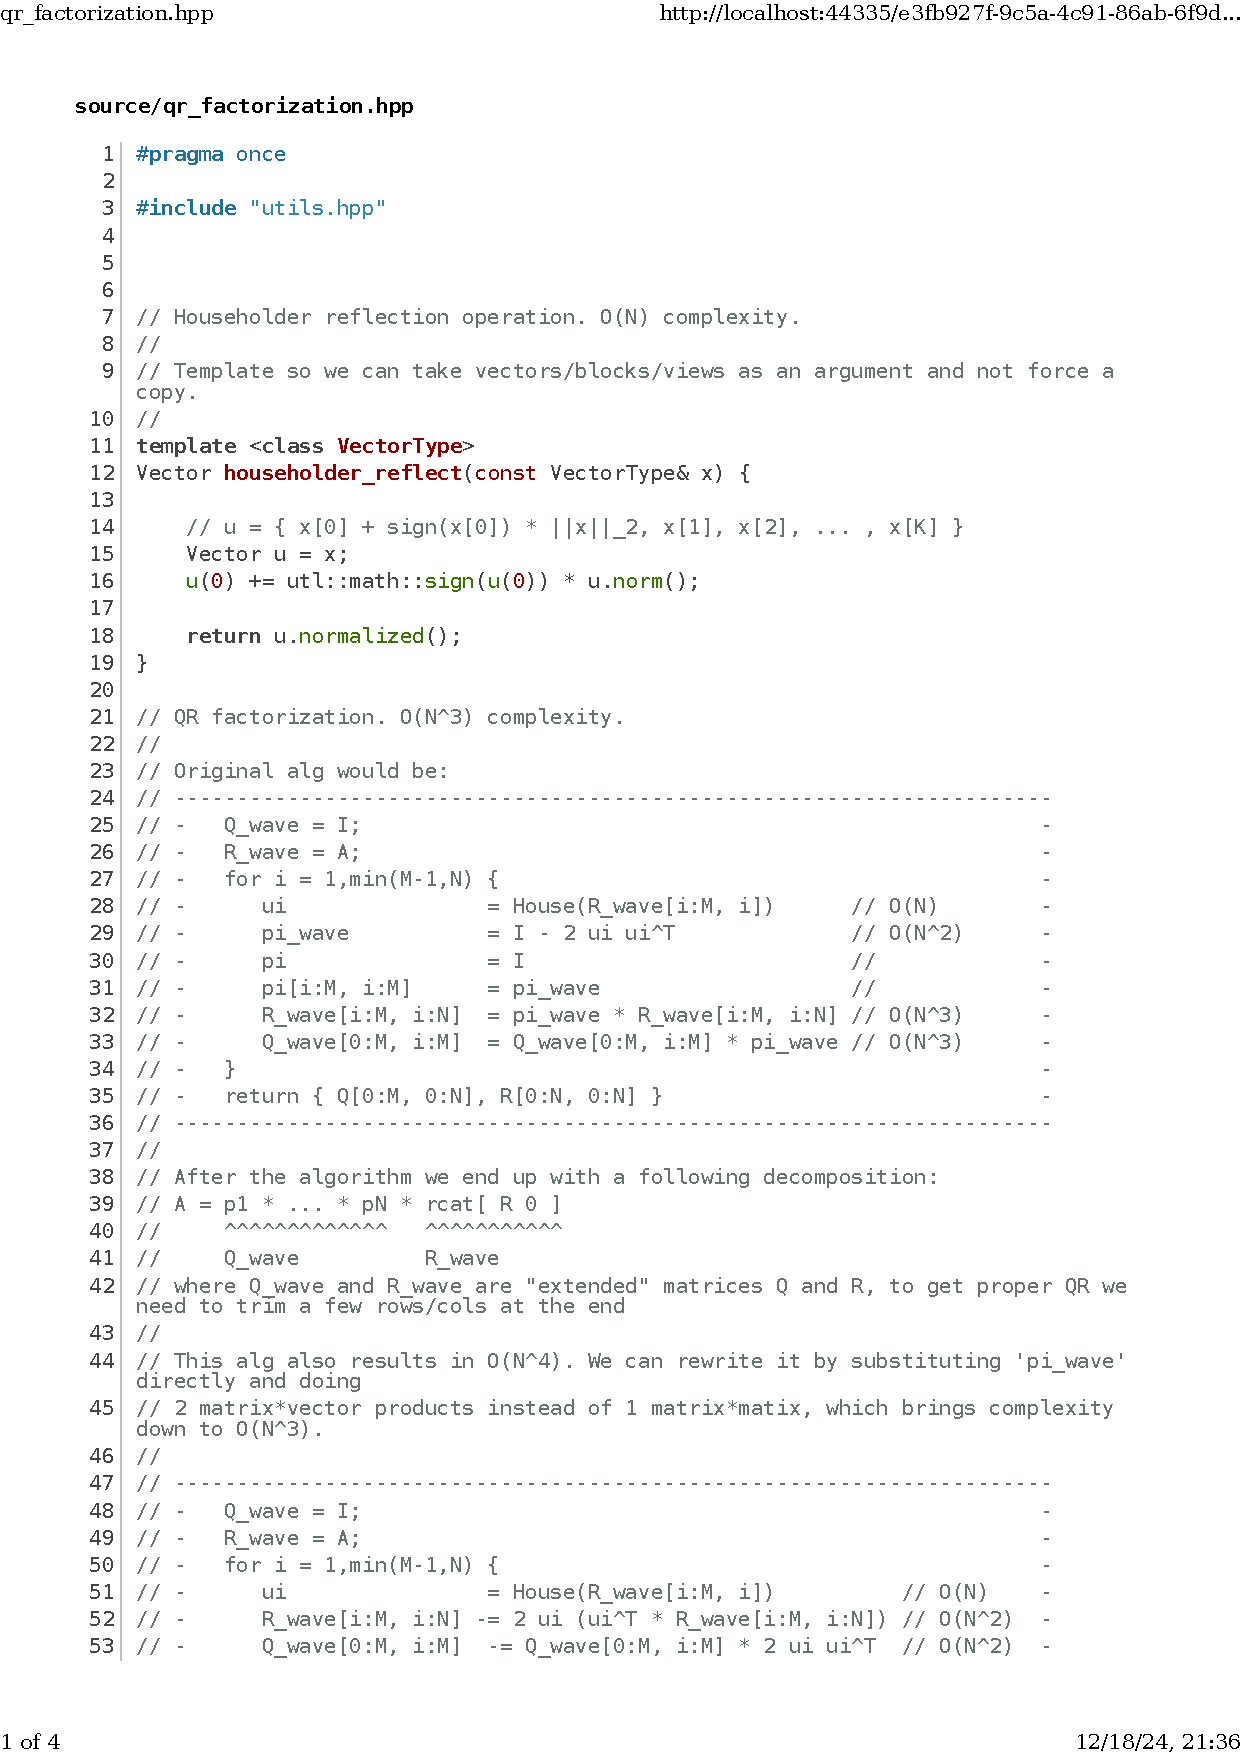
\includepdf[scale=0.9, pages=-]{images/qr_factorization.hpp.pdf}
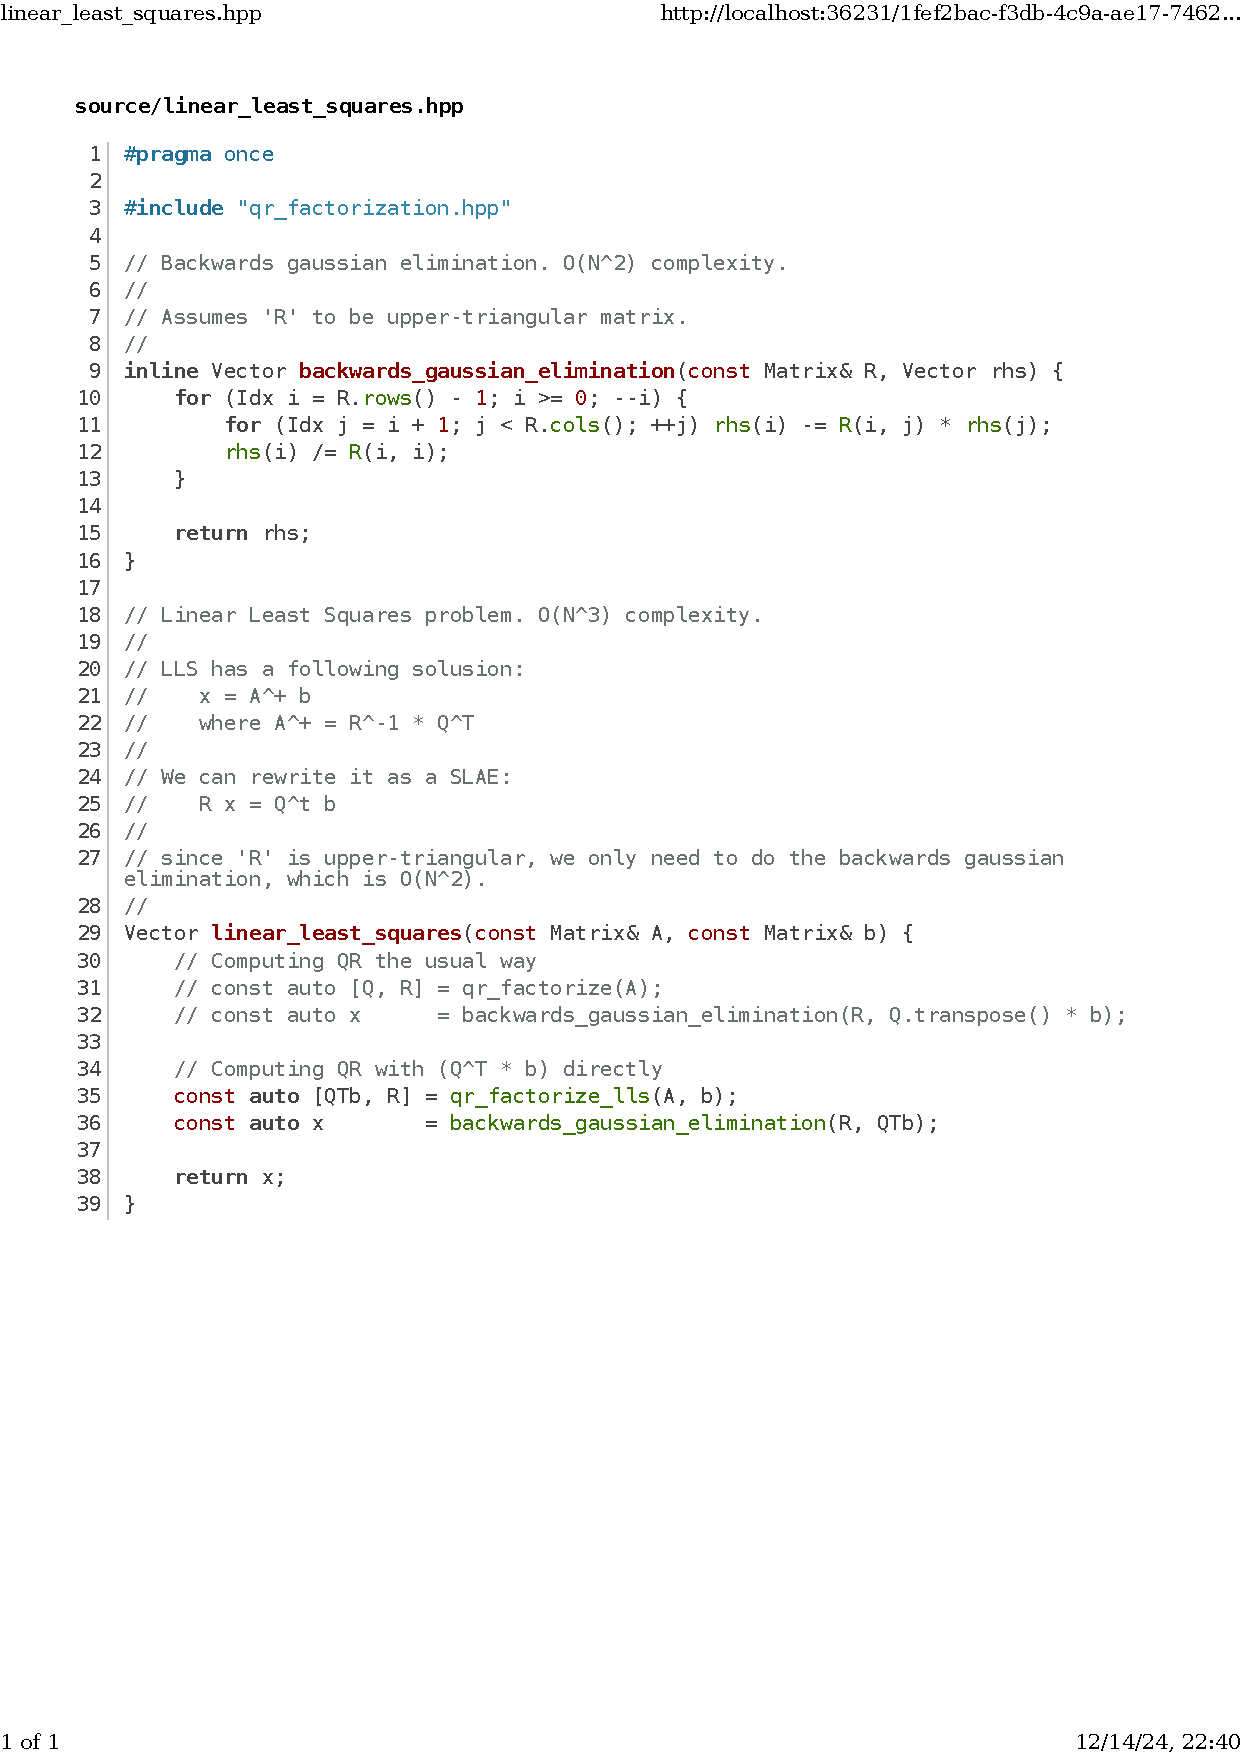
\includepdf[scale=0.9, pages=-]{images/linear_least_squares.hpp.pdf}
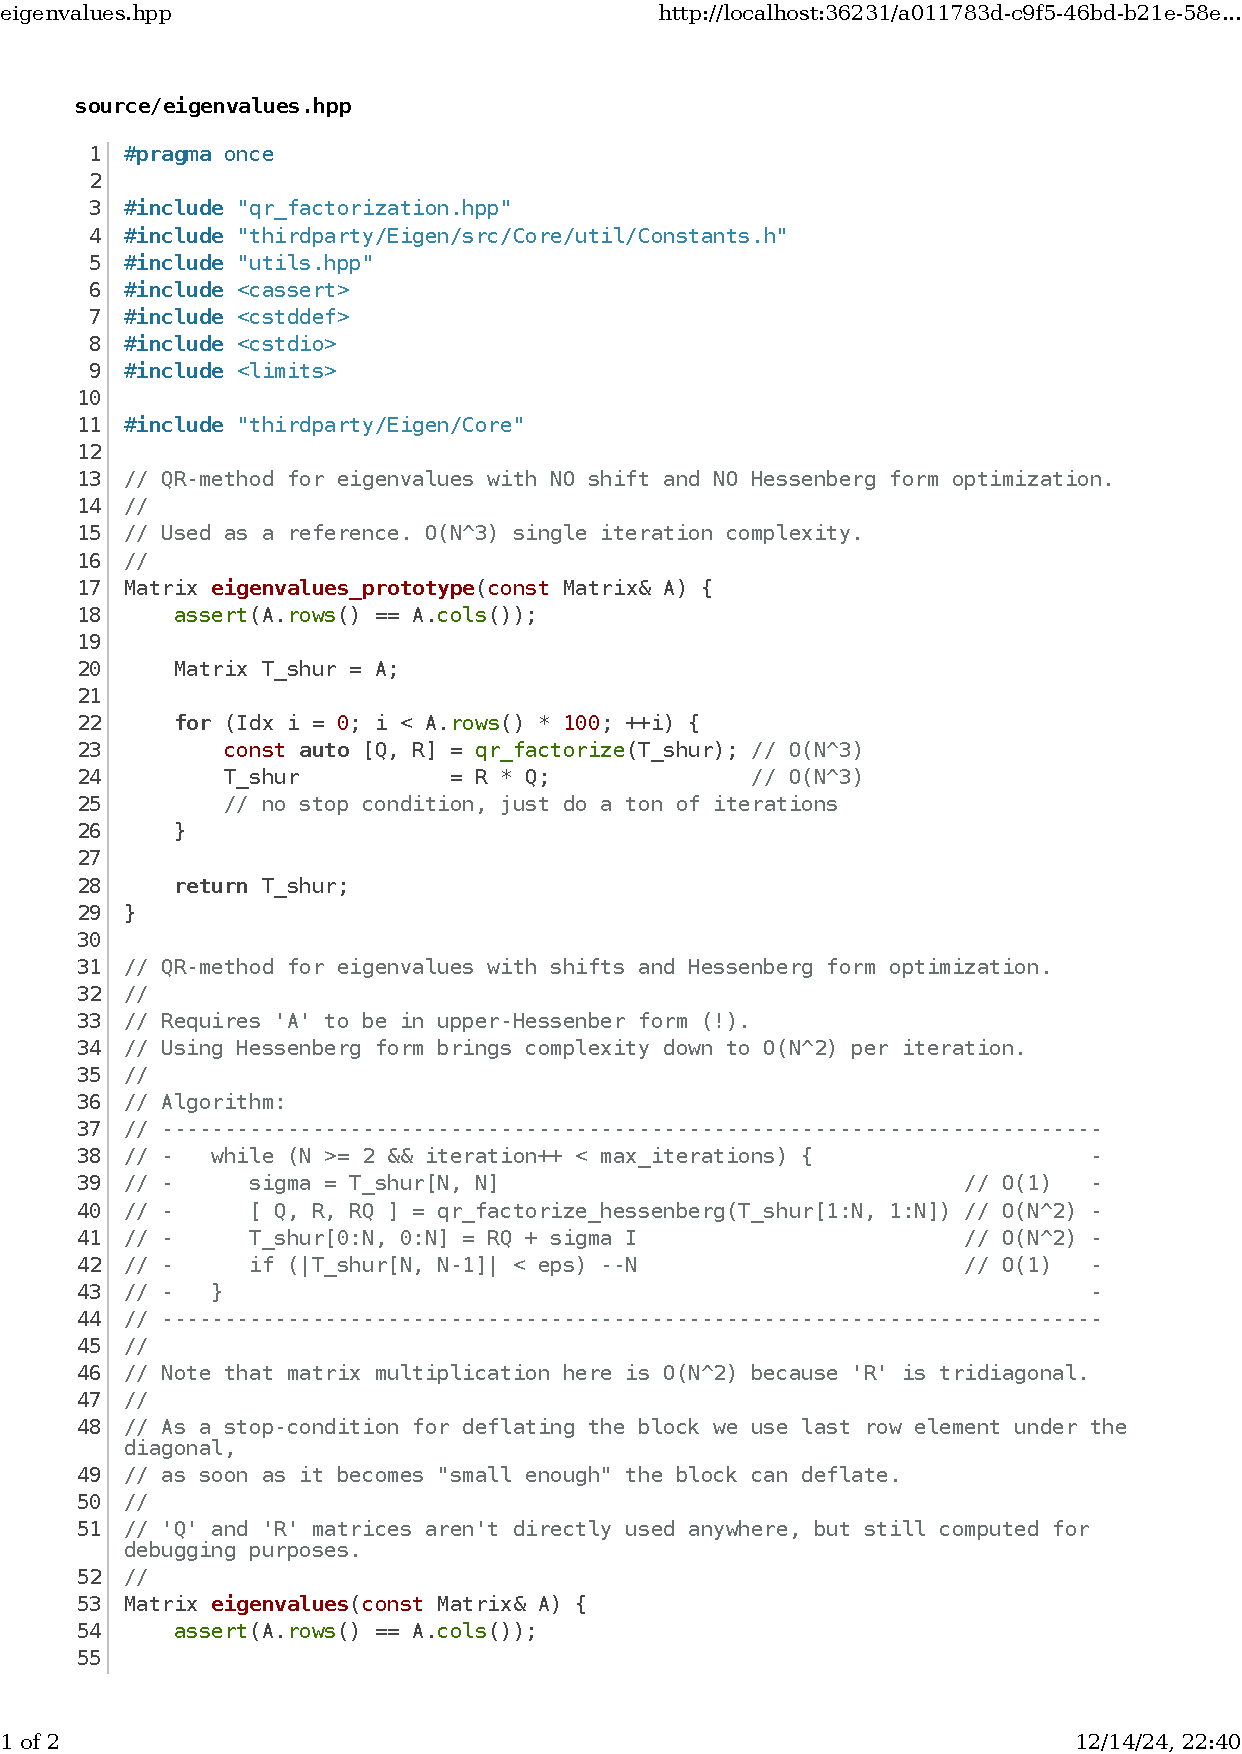
\includepdf[scale=0.9, pages=-]{images/eigenvalues.hpp.pdf}
\includepdf[scale=0.9, pages=-]{images/main.hpp.pdf}

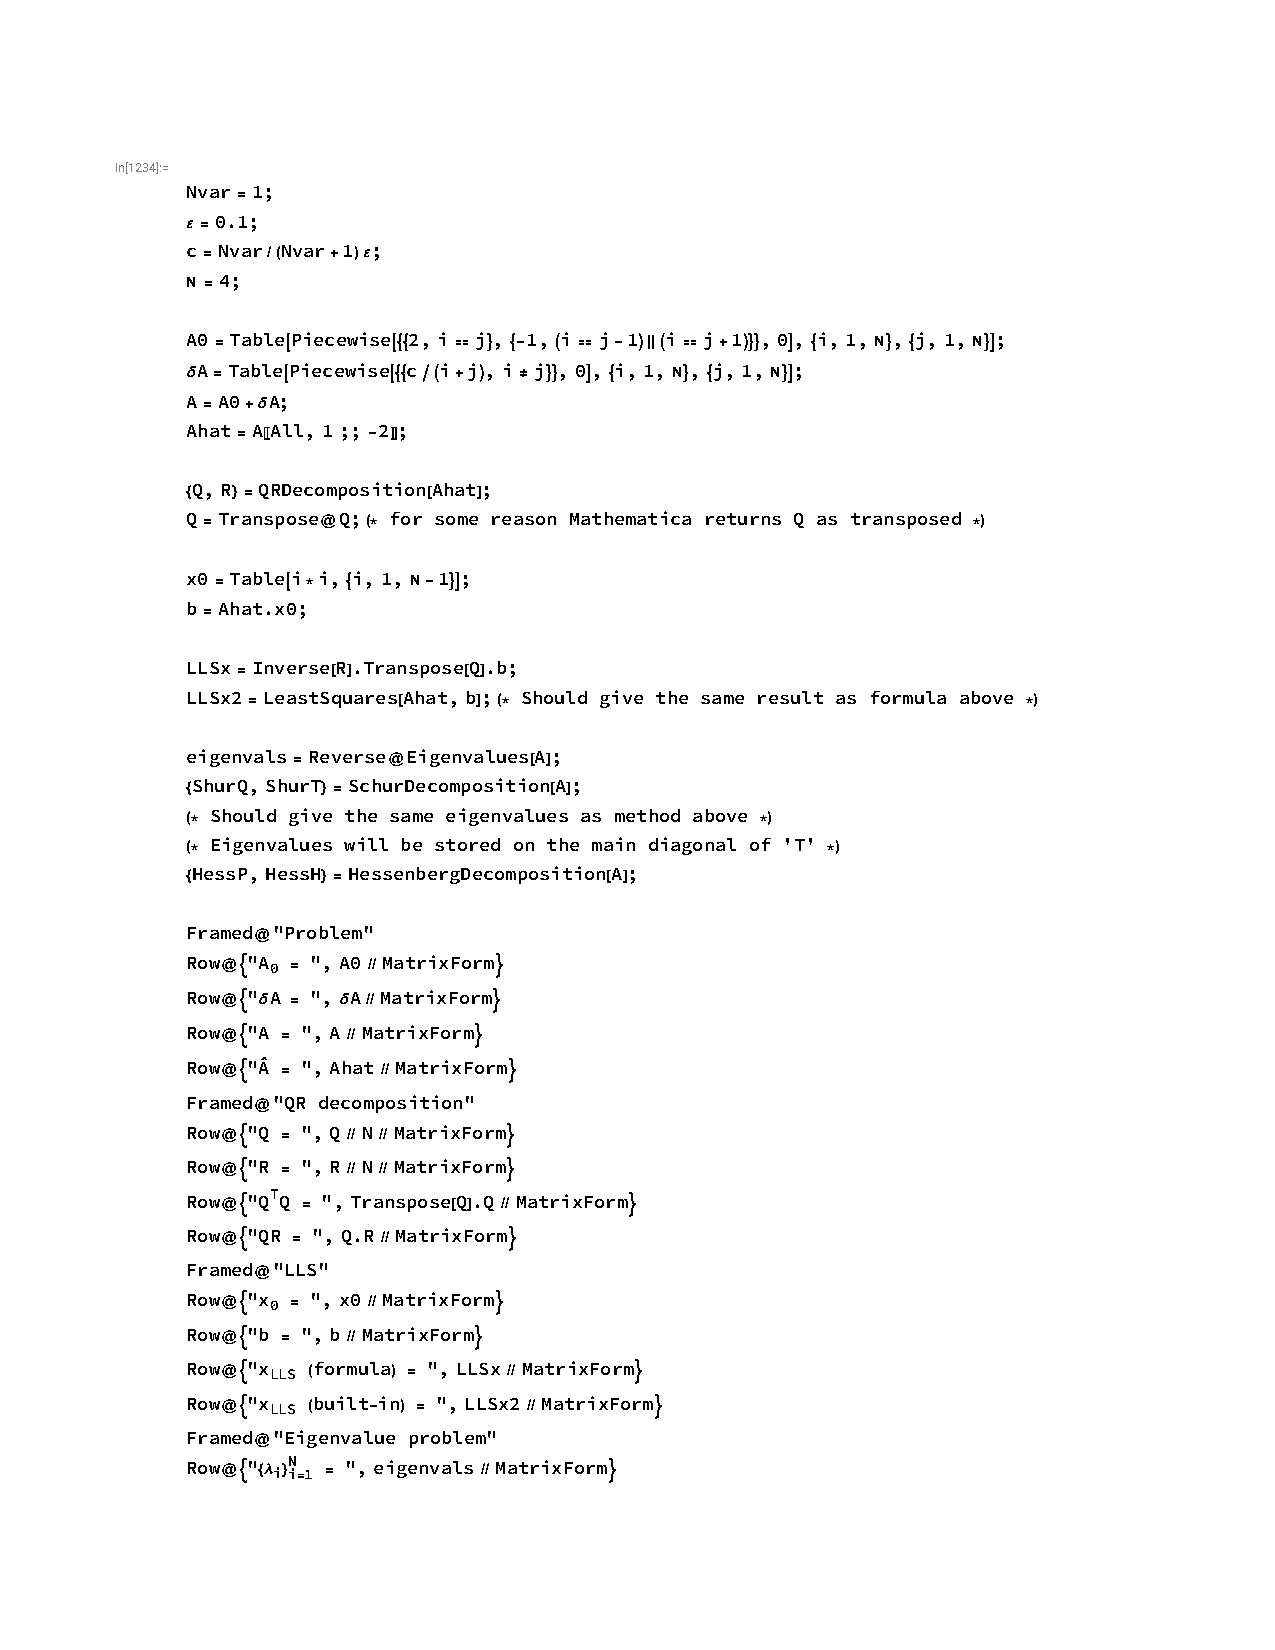
\includepdf[scale=0.9,pagecommand=\section{Листинг проверочного скрипта на Wolfram Mathematica}]{images/mathematica.pdf}

\section{Приложение. Пример сводки результатов расчетной программы}

\begin{tinyverbatim}
---------------
--- Problem ---
---------------

epsilon -> 1e-06
N       -> 4
A0      -> Tensor [size = 16] (4 x 4):
  [  2 -1  0  0 ]
  [ -1  2 -1  0 ]
  [  0 -1  2 -1 ]
  [  0  0 -1  2 ]

deltaA  -> Tensor [size = 16] (4 x 4):
  [           0 1.66667e-07    1.25e-07       1e-07 ]
  [ 1.66667e-07           0       1e-07 8.33333e-08 ]
  [    1.25e-07       1e-07           0 7.14286e-08 ]
  [       1e-07 8.33333e-08 7.14286e-08           0 ]

A       -> Tensor [size = 16] (4 x 4):
  [        2          -1 1.25e-07       1e-07 ]
  [       -1           2       -1 8.33333e-08 ]
  [ 1.25e-07          -1        2          -1 ]
  [    1e-07 8.33333e-08       -1           2 ]

A_hat   -> Tensor [size = 12] (4 x 3):
  [        2          -1 1.25e-07 ]
  [       -1           2       -1 ]
  [ 1.25e-07          -1        2 ]
  [    1e-07 8.33333e-08       -1 ]

------------------------
--- QR factorization ---
------------------------

Q             -> Tensor [size = 12] (4 x 3):
  [    -0.894427    -0.358569 -0.19518 ]
  [     0.447214    -0.717137 -0.39036 ]
  [ -5.59017e-08     0.597614 -0.58554 ]
  [ -4.47214e-08 -9.76103e-08  0.68313 ]

R             -> Tensor [size = 9] (3 x 3):
  [     -2.23607      1.78885 -0.447214 ]
  [  2.22045e-16     -1.67332   1.91237 ]
  [ -2.64698e-23 -1.11022e-16  -1.46385 ]

Verification:

Q^T * Q       -> Tensor [size = 9] (3 x 3):
  [           1  2.77556e-16  8.32667e-17 ]
  [ 2.77556e-16            1 -2.22045e-16 ]
  [ 8.32667e-17 -2.22045e-16            1 ]

Q * R - A_hat -> Tensor [size = 12] (4 x 3):
  [  2.22045e-15 -1.77636e-15  6.83606e-16 ]
  [ -8.88178e-16 -8.88178e-16  1.33227e-15 ]
  [  1.32697e-16  3.33067e-16 -4.44089e-16 ]
  [  3.97047e-23 -7.58428e-17  2.22045e-16 ]

-------------------------------------
--- Linear Least Squares solution ---
-------------------------------------

x0                 -> Tensor [size = 3] (3 x 1):
  [ 1 ]
  [ 4 ]
  [ 9 ]

b                  -> Tensor [size = 4] (4 x 1):
  [ -2 ]
  [ -2 ]
  [ 14 ]
  [ -9 ]

x_lls              -> Tensor [size = 3] (3 x 1):
  [ 1 ]
  [ 4 ]
  [ 9 ]

lls_error_estimate -> 1.8496162997539822e-16

---------------------------
--- Eigenvalue solution ---
---------------------------

H_hessenberg                  -> Tensor [size = 16] (4 x 4):
  [           2            1 -2.64698e-23  1.32349e-23 ]
  [           1            2           -1 -2.64698e-23 ]
  [ 2.64698e-23           -1            2            1 ]
  [ 1.32349e-23 -2.64698e-23            1            2 ]

T_shur                        -> Tensor [size = 16] (4 x 4):
  [     3.61803 -1.46354e-16 -1.55722e-16 -1.88824e-16 ]
  [ 2.56137e-27     0.381966  4.50213e-16  3.42274e-16 ]
  [ 6.03553e-17  1.73417e-16      2.61803 -4.28483e-16 ]
  [ 1.15867e-17  1.13712e-16 -8.62537e-22      1.38197 ]

lambda0 (analythic eigenvals) -> Tensor [size = 4] (4 x 1):
  [ 0.381966 ]
  [  1.38197 ]
  [  2.61803 ]
  [  3.61803 ]

lambda    (numeric eigenvals) -> Tensor [size = 4] (4 x 1):
  [ 0.381966 ]
  [  1.38197 ]
  [  2.61803 ]
  [  3.61803 ]

z0      (analythic eigenvecs) -> Tensor [size = 16] (4 x 4):
  [ 0.371748  0.601501  0.601501  0.371748 ]
  [ 0.601501  0.371748 -0.371748 -0.601501 ]
  [ 0.601501 -0.371748 -0.371748  0.601501 ]
  [ 0.371748 -0.601501  0.601501 -0.371748 ]

|----|-------------------------|-------------------------|
|  j | |lambda_j^0 - lambda_j| |        ||z0_j - z-j||_2 |
|----|-------------------------|-------------------------|
|   1|              2.99649e-07|                        x|
|   2|              8.66901e-08|                        x|
|   3|              9.96489e-08|                        x|
|   4|              1.13310e-07|                        x|
\end{tinyverbatim}

\end{document}
